\section{The \lang language}

We now present a formalization of the \lang language featuring
a minimal ML language with let-polymorphism, abstract types, pairs, and our novel
linear type system with borrows which uses kinds and qualified types.
For ease of presentation,
our formalization makes the following simplifications.
First, we only consider matching on pairs, instead of arbitrary algebraic
datatypes. We consider separate operators for borrowing and reborrowing (taking
the borrow of a borrow). We consider regions to be fully annotated
and present a set of rules to infer their placement.
Finally we emulates region variables
as a series of nesting indices.

In the rest of this section, we present the syntax (\cref{syntax}),
a linearity-aware semantics (\cref{sem}), syntax directed typing rules
(\cref{sdtyping}) and automatic rules for region annotations (\cref{regionannot}).

\subsection{Syntax}
\label{syntax}

The syntax of \lang is presented in \cref{grammar} and follows
traditional ML languages with let bindings.
Data constructors are introduced by $\introK{K}{e}$ and eliminated
with by $\elimK{K}{e}$.
Types are composed of type variable $\tvar$, parameterized type constructors
$\T{t}$ and arrow types annotated with a kind, noted $\tau \tarr{k} \tau$.
Kinds can be either a kind variable $\kvar$, affine $\kaff$ or unrestricted $\kun$.
Type schemes and kind schemes are guarded by a set of constraints.

Environments are composed of value and type bindings, along with type
declarations. Type declarations, of the form
$\tydecl{t}{\kschm}{K}{\tau}$, introduce both a new type constructor $\T{t}$ and
a data constructor $K$.

\begin{figure*}[t]
  \centering
  \begin{subfigure}[t]{0.45\linewidth}
\begin{align*}
  \htag{Expressions}
  e ::=&\ c \mid x \mid \app{e}{e'} \mid \lam{x}{e} \mid \letin{x}{e}{e'}\\
  % |&\ \fix{e}\tag{Fixpoint}\\
  |&\ \introPair{e}{e'} \mid \matchin{x,y}{e}{e'}\tag{Pairs}\\
  |&\ \region{x}{e}\tag{Region}\\
  |&\ \borrow{x}\tag{Borrows}\\
  % |&\ \introK{K}{e}\tag{Data Constructor introduction}\\
  % |&\ \elimK{K}{e}\tag{Data Constructor elimination}\\
  \htag{Environments}
  \E ::=&\ b^*\\
  b ::=&\ \bvar{x}{\schm}\tag{Variable bindings}\\
  |&\ \bvar{\tvar}{\kschm}\tag{Type bindings}\\
  % |&\ \tydecl{t}{\kschm}{K}{\tau}\tag{Type Declaration}\\
  \htag{Type and kind Schemes}
  \schm ::=&\ \forall\kvar^*\forall\bvar{\alpha}{k}^*.(\qual{C}{\tau})\\
  \kschm ::=&\ \forall\kvar^*.(\qual{C}{k_i^* \karr k})\\
\end{align*}
\end{subfigure}\hfill
\begin{subfigure}[t]{0.5\linewidth}
\begin{align*}
  \htag{Type Expressions}
  \tau ::=&\ \tvar\tag{Type variables}\\
  |&\ \tau\tarr{k}\tau\tag{Function types}\\
  |&\ \tapp{t}{\tau^*}\tag{Type constructors}\\
  |&\ \borrow{\tau}\tag{Borrowed Type}\\
  \htag{Kinds}
  k ::=&\ \kvar\tag{Kind variables}\\
  |&\ \klin_n\tag{Linear kind}\\
  |&\ \kaff_n\tag{Affine kind}\\
  |&\ \kun_n\tag{Unrestricted kind}\\
  n \in&\ \mathbb N \cup \{\infty\}\\
  \htag{Constraints}
  C ::= (\Cleq{k}{k'})^*
\end{align*}
\end{subfigure}

%%% Local Variables:
%%% mode: latex
%%% TeX-master: "main"
%%% End:

  \caption{Syntax}
  \label{grammar}
\end{figure*}
\begin{figure}[!tbp]
%   \begin{align*}
% \end{align*}
% \begin{minipage}[t]{0.49\linewidth}
  \begin{align*}
    \htag{Elaborated expressions}
    v ::=~& x \mid \ivar x {\Multi k} {\Multi\tau} \mid \lam[k]{x}{e} \mid \introPair[k]{v}{v'}\\
    e ::=~& x \mid \ivar x {\Multi k} {\Multi\tau} \mid \lam[k]{x}{e} \mid \introPair[k]{e}{e'}\\
    \mid~& \matchin{x,y}{e}{e'} \tag{Tagged pairs}\\
    \mid~& \letin{x}{e}{e'}\\
    \mid~& \letin{\bvar x \schm}{v}{e'}\\
    \mid~& \iapp{\Sp}{e}{e'} \tag{El. application}\\
    \mid~& \region{\Sone x\BORROW}{e}\tag{Region}\\
    \mid~& \borrow{x} \mid \reborrow{x}\tag{Borrows}\\
    \mid~& \create \mid \observe \mid \update \mid \destroy \tag{Resources}\\
    % e &::= \dots \\
    % &\mid \ilam{\Multi\kvar}{\Multi{\tvar : k}}Ckx{\tau}e \tag{El. poly abstraction} \\
    % &\mid \imlam kx{\tau}e \tag{El. mono abstraction} \\
    % &\mid \ivar x {\Multi k} {\Multi\tau} \tag{Instantiation} \\
    % &\mid \introPair[k]{e}{e} \tag{Tagged pairs}\\
    % &\mid \iapp{\Sp}{e}{e} \tag{El. application}\\
    \htag{Elaborated A-normal expressions}
    % TODO: what about constructors applied to values?
    X ::=~& x \mid \ivar x {\Multi k} {\Multi\tau}\\
    v ::=~& c \mid X \mid \lam[k]{x}{e} \mid \introPair[k]{X}{X'}\\
    E ::=~& c \mid X \mid \lam[k]{x}{e} \mid \introPair[k]{x}{x'}\\
    \mid~& \borrow{x} \mid \reborrow{x}\tag{Borrows}\\
    \mid~& \create \mid \observe \mid \update \mid \destroy \tag{Resources}\\
    \mid~& \app{x}{x'} \tag{El. application}\\
    e ::=~& \letin{x}{E}{e'}\\
    \mid~& \letin{\bvar x \schm}{v}{e'}\\
    \mid~& \matchin{x,y}{z}{e} \tag{Tagged pairs}\\
    \mid~& \region{\Sone x\BORROW}{e}\tag{Region}\\
    \htag{Environment}
    \Addr ::=~& \Multi\IBORROW\Multi\MBORROW\Loc \tag{Locations}
    % \\           &\mid \borrow{\Addr} \tag{Borrows}
    \\
    \Perm ::=~& \{\} \mid \Perm + \Addr \tag{Permissions}
    \\
    r ::=~& \Addr \mid c \tag{Results}\\
    \VEnv ::=~& \Eempty \mid \VEnv( x \mapsto r) \tag{Enviroments} \\
%   \end{align*}
% \end{minipage}
% \hfill
% \begin{minipage}[t]{0.49\linewidth}
%   \begin{align*}
    \htag{Storables}
    w ::=~& \StPClosure \VEnv {\Multi\kvar} C k x e \tag{Poly Closures}\\
    \mid~& \StClosure \VEnv k x e \tag{Closures} \\
    \mid~& \StPair k r r \tag{Pairs} \\
    \mid~& \StRes r \tag{Resources} \\
    \mid~& \StFreed \tag{Freed Resource}
    \\
    \htag{Store}
    \Store ::=~& \Eempty \mid \Store( \Loc \mapsto w)
    \\
    \htag{Splittings}
    \Sp ::=~& \Multi{\SpBoth \mid \SpBorrow \mid \SpLeft \mid \SpRight \mid \SpSusp \mid \SpSuspB}
  \end{align*}
% \end{minipage}
\caption{Syntax of internal language}
\label{fig:syntax-internal-language}
\end{figure}

%%% Local Variables:
%%% mode: latex
%%% TeX-master: "main"
%%% End:


\clearpage
\subsection{Semantics}
\label{sem}

\begin{figure*}[ht]
  % \begin{mathpar}
  \inferrule[Lam]
  { j \fresh }
  { \ered{\closure{j}{x}{e}}{\emptyset}{\lam{x}{e}}{\closure{j}{x}{e}} }
  \and
  \inferrule[App]
  { \ered{I}{E}{f}{\closure{j}{x}{e_f}} \\
    \ered{I'}{E'}{e}{v} \\
    \ered{I''}{E''}{\subst{x}{v}{e_f}}{v_f}
  }
  { \ered{I,I',I''}{E,E',E'',\closure{j}{x}{e_f}}{\app{f}{e}}{v_f} }
  \and
  \inferrule[Let]
  { \ered{I}{E}{e}{v} \\
    \ered{I'}{E'}{\subst{x}{v}{e'}}{v'}
  }
  { \ered{I,I'}{E,E'}{\letin{x}{e}{e'}}{v'} }
\end{mathpar}
%%% Local Variables:
%%% mode: latex
%%% TeX-master: "main"
%%% End:

    \begin{mathpar}
    \inferrule{}{ \Sigma, \rho \vdash c \Downarrow \Sigma, c}

    \inferrule{}{\Sigma, \rho \vdash x \Downarrow \Sigma, \rho(x)}

    \inferrule{
      \Sigma, \rho \vdash e \Downarrow \Loc \\
      \Sigma (\Loc) = (\rho, \ilam {\kvar^*}{\tvar^*}Ckx{e}) \\\\
      \Sigma' =  \entail C {(\kaff \le k)} \Rightarrow
      \Sigma[\Loc\mapsto\blob] ; \Sigma \\
      \Loc'\notin\Dom\Sigma'  \\
      \Sigma'' = \Sigma[\Loc' \mapsto (\rho,\lam[{k[\kvar^*\mapsto k^*]}]xe) ]
    }{\Sigma, \rho \vdash  \ivar e{k^*}{\tau^*}  \Downarrow \Sigma'', \Loc'
    }

    \inferrule{
      \Loc\notin\Dom\Sigma \\
      \Sigma' = \Sigma[\Loc \mapsto (\rho, \ilam  {\kvar^*}{\tvar^*}Ck xe)]
    }{
      \Sigma, \rho \vdash \ilam  {\kvar^*}{\tvar^*}Ck xe \Downarrow \Sigma', \Loc
    }
    
    \inferrule{
      \Sigma, \rho \vdash e \Downarrow \Sigma', \Loc \\
      \Sigma' (\Loc) = (\rho'',\lam[k]{x}{e''}) \\
      \Sigma'' = \entail {} {(\kaff \le k)} \Rightarrow \Sigma'[\Loc\mapsto\blob];\Sigma'\\
      \Sigma'', \rho \vdash e' \Downarrow \Sigma''', r' \\
      \Sigma''', \rho''[x\mapsto r'] \vdash e'' \Downarrow \Sigma'''', r
    }{\Sigma, \rho \vdash \app{e}{e'} \Downarrow \Sigma'''', r}

    \inferrule{
      \Sigma, \rho \vdash e \Downarrow \Sigma', r \\
      \Sigma', \rho[x \mapsto r] \vdash e' \Downarrow \Sigma'', r'
    }{
      \Sigma, \rho \vdash \letin{x}{e}{e'} \Downarrow \Sigma'', r'
    }

    \inferrule{
      \Sigma, \rho \vdash e \Downarrow \Sigma', r \\
      \Sigma', \rho \vdash e' \Downarrow \Sigma'', r' \\
      \Loc\notin\Dom{\Sigma''} \\
      \Sigma''' = \Sigma''[\Loc \mapsto (r, r')]
    }{
      \Sigma, \rho \vdash \introPair{e}{e'} \Downarrow \Sigma''', \Loc
    }

    \inferrule{
      \Sigma, \rho \vdash e \Downarrow \Sigma', \Loc \\
      \Sigma' (\Loc) = (r, r') \\
      \Sigma', \rho[x,y \mapsto r, r'] \vdash e' \Downarrow \Sigma'', r''
    }{
      \Sigma, \rho \vdash \matchin{x,y}{e}{e'} \Downarrow  \Sigma'', r''
    }

    \inferrule{
      \rho (x) = \alpha \\
      \Sigma (\alpha) = W \\
      (\Sigma\setminus\alpha)[\borrow{\alpha} \mapsto W], \rho \vdash e
      \Downarrow \Sigma', r \\
      \Sigma'' = (\Sigma' \setminus\borrow{\alpha})[\alpha \mapsto W]
    }{
      \Sigma, \rho \vdash \region{x}{e} \Downarrow \Sigma', r
    }

    \inferrule{\rho (x) = \alpha}{
      \Sigma, \rho \vdash \borrow{x} \Downarrow \Sigma, \borrow\alpha
    }
    \\
    \inferrule{
      \Sigma, \rho \vdash e \Downarrow \Sigma', r\\
      \Loc\notin \Dom\Sigma' }{
      \Sigma,\rho \vdash \create e \Downarrow \Sigma'[\Loc \mapsto \rss{r}], \Loc
    }

    \inferrule{
      \Sigma, \rho \vdash e \Downarrow \Sigma', \Loc \\
      \Sigma' (\Loc) = \rss{r}
    }{
      \Sigma, \rho \vdash \destroy e \Downarrow \Sigma'[\Loc\mapsto \blob], ()
    }

    \inferrule{
      \Sigma, \rho \vdash e \Downarrow \Sigma', \borrow[i]\alpha \\
      \Sigma' (\borrow[i]\alpha) = \rss{r}
    }{
      \Sigma, \rho \vdash \observe e \Downarrow \Sigma', r
    }

    \inferrule{
      \Sigma, \rho \vdash e \Downarrow \Sigma', \borrow[m]\alpha \\
      \Sigma', \rho \vdash e' \Downarrow \Sigma'', r' \\
      \Sigma'' (\borrow[m]\alpha) = \rss{r} \\
      \Sigma''' = \Sigma''[\borrow[m]\alpha \mapsto r']
    }{
      \Sigma, \rho \vdash \update e {e'} \Downarrow \Sigma''', ()
    }

  \end{mathpar}
  \caption{Reduction rules -- $\Sigma, \rho \vdash e \Downarrow
    \Sigma', r$ }
  \label{fig:reduction}
\end{figure*}


%%% Local Variables:
%%% mode: latex
%%% TeX-master: "main"
%%% End:

\begin{figure}
  \lstsemrule{varinst}
  \medskip
  \lstsemrule{sapp}
  \medskip
  \lstsemrule{spair}
  \medskip
  \lstsemrule{sregion}
  \caption{Big-step Interpretation}
\end{figure}


%%% Local Variables:
%%% mode: latex
%%% TeX-master: "main"
%%% End:


\clearpage
\subsection{Typing}
\label{sdtyping}

\subsubsection{Constraint language}

\newcommand\A{\mathcal A}
\newcommand\SC{\mathcal S}

Let us note $\A$ our constraint system. The grammar of constraints is
given in  \cref{grammar:constraint}.
$\A$ is defined as the smallest cylindric term constraint system that
satisfies the axiom shown in \cref{rules:entail}.
We follows the traditional HM(X) formulation
with conjunctions, projections and type inequalities.
The new element specific to our approach are kind inequalities.
Entailment is noted $\entail{C}{D}$, where $D$ is a consequence of the
constraints $C$.
We say that $C$ and $D$ are equivalent, noted $C \equivC D$,
when $\entail{C}{D}$ and $\entail{D}{C}$.
\TODO{Give the cylindric properties ?}

\begin{figure}[tp]
  \centering
  \begin{align*}
    C &::= \Cleq{\tau_1}{\tau_2}
        \mid \Cleq{k_1}{k_2}
        \mid C_1 \Cand C_2
        \mid \Cproj{\tvar}{C}
        \mid \Cproj{\kvar}{C}
  \end{align*}
  \caption{The constraint language}
  \label{grammar:constraint}
\end{figure}

\begin{figure*}[tp]
  \begin{minipage}{0.65\linewidth}
  \begin{mathpar}
    \inferrule[Lat-UAL]{}{\kun \lk \kaff \lk \klin}
    \and
    \inferrule[Lat-Level]{\mul \lk \mul' \and n \lk n'}{\mul_n \lk_\Lat \mul'_{n'}}
  \end{mathpar}
\end{minipage}~
\begin{minipage}{0.2\linewidth}
  \centering
  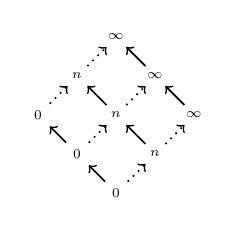
\begin{tikzpicture}
    [->,auto,semithick, every node/.style={scale=0.7}]
    \node(U) {$\kun_0$} ;
    \node(A) [above left of=U] {$\kaff_0$} ;
    \node(L) [above left of=A] {$\klin_0$} ;
    \node(Un) [above right of=U] {$\kun_n$} ;
    \node(An) [above left of=Un] {$\kaff_n$} ;
    \node(Ln) [above left of=An] {$\klin_n$} ;
    \node(Uinf) [above right of=Un] {$\kun_\infty$} ;
    \node(Ainf) [above left of=Uinf] {$\kaff_\infty$} ;
    \node(Linf) [above left of=Ainf] {$\klin_\infty$} ;
    \path
    (U) edge (A)
    (A) edge (L)
    (Un) edge (An)
    (An) edge (Ln)
    (Uinf) edge (Ainf)
    (Ainf) edge (Linf)
    ;
    \path[dotted]
    (U) edge (Un)
    (A) edge (An)
    (L) edge (Ln)
    (Un) edge (Uinf)
    (An) edge (Ainf)
    (Ln) edge (Linf)
    ;
  \end{tikzpicture}
\end{minipage}

%%% Local Variables:
%%% mode: latex
%%% TeX-master: "../main"
%%% End:

  \caption{Lattice inequalities -- $k \lk_\Lat k'$}
  \begin{mathpar}
  \inferrule
  {}{ \entail{}{\Cleq{\kvar}{\kaff}} }
  \and
  \inferrule
  {}{ \entail{}{\Cleq{\kun}{\kvar}} }
  \and
  \inferrule
  {}{ \entail{}{\Cleq{\kvar}{\kvar}} }
  \and
  % \inferrule
  % {\Cleq{k}{k'} \in C}{ \entail{C}{\Cleq{k}{k'}} }
  % \and
  % \inferrule
  % { \entail{C}{\Cleq{x_1}{x}}\\
  %   \entail{C}{\Cleq{x}{x_2}}
  % }
  % { \entail{C}{\Cleq{x_1}{x_2}} }
  % \and
  % \inferrule
  % { \entail{C}{D} }
  % { \entail{C}{\Cproj{x}{D}} }
  % \\
  \inferrule
  { \entail{C}{\Cleq{\tau'_1}{\tau_1}}\\
    \entail{C}{\Cleq{\tau_2}{\tau'_2}}\\
    \entail{C}{\Cleq{k}{k'}}
  }
  { \entail{C}{\Cleq{\tau_1\tarr{k}\tau_2}{\tau'_1\tarr{k'}\tau'_2}} }
  \and
  \inferrule
  { \forall i,\ \entail{C}{\Cleq{\tau_i}{\tau_i}}\\
  }
  { \entail{C}{\Cleq{\tapp{t}{(\tau_i)}}{\tapp{t}{(\tau'_i)}}} }
  \and
  
  % \and
  % \inferrule
  % { \entail{C}{\Cleq{k}{k'}} \\
  %   \entail{C}{\Cleq{k'}{k}} }
  % { \entail{C}{\Ceq{k}{k'}} }
  % \and
  % \inferrule
  % { \entail{C}{\Cleq{k}{k'}} }
  % { \entail{C}{\Ckind{\tau_0\tarr{k}\tau_1}}{k'}}
  % \and
  % \text{Completion to form a cylindric constraint system.}
\end{mathpar}

%%% Local Variables:
%%% mode: latex
%%% TeX-master: "../main"
%%% End:

  \caption{Base entailment rules -- $\entail{C}{D}$ }
  \label{rules:entail}
\end{figure*}


We note $\SC$ the set of solved forms
which can be used inside type and kind schemes.
We define $\SC$ as $\A$ quotiented by the relation $\equivC$.
%
We consider the existence of a function $\operatorname{normalize}$ which takes
a constraint in $\A$ and a substitution $\psi$ and returns a constraint
in solved form $C' \in \SC$,
and an updated substitution. We detail the implementation
of the normalization function in \cref{sec:normalize}

% $\mathcal S$ is composed only of kind
% inequalities \emph{over variables}. For convenience, if $C\in\mathcal S$, we
% note $C$ as a list of kind inequalities: $\Cleq{\kvar_i}{\kvar_{i'}}^n$.
% \TODO{Extend the properties of solved forms}

\subsubsection{Kinding}


\begin{figure}[ht]
  \centering
  \begin{mathpar}
  \inferrule[KVar]
  { \bvar{\tvar}{k} \in \E }
  { \inferSK{C}{\E}{\tvar}{k}
  }
  \and
  \inferrule[KPair]
  { \forall i \quad
    \inferSK{C}{\E}{\tau_i}{k_i} \quad
    \inferSS{C}{\E}{k_i}{k}
  }
  { \inferSK{C}{\E}{\tyPair{\tau_1}{\tau_2}}{k} }
  \and
  \inferrule[KApp]
  { \bvar{\T{\tcon}}{
      \forall \Multi[i]\kvar.\ \qual{D}{(\Multi[j]{k'}) \karr k'}}
    \in \E \\
    \unif = \subst{\Multi[i]\kvar}{\Multi[i]k}{} \\
    \entail C {\unif D} \\
    \forall j\quad
    \inferSK{C}{\E}{\tau_j}{k_j}\quad
    \inferSS{C}{\E}{k_j}{\unif{k'_j}}
  }
  { \inferSK{C}{\E}{\tapp{\tcon}{\Multi[j]{\tau}}}{\unif{k'}} }
  \and
  \inferrule[KBorrow]
  {}{ \inferSK{C}{\E}{\borrowty{k}{\tau}}{k}}
  \and
  \inferrule[KArr]
  {}
  { \inferSK{C}{\E}{\tau_1 \tarr{k} \tau_2}{k} }
\end{mathpar}


%%% Local Variables:
%%% mode: latex
%%% TeX-master: "../main"
%%% End:

  \caption{Syntax-directed kind inference --
    $\inferSK{C}{\E}{\tau}{(\Multi k)k}$}
  \label{rules:sd-kinding}
\end{figure}

\subsubsection{Environments}


\begin{figure}[tp]
  \begin{mathpar}
  \inferrule[ESplit-Empty]{}{
    \bsplit{\Cempty}\Eempty\Eempty\Eempty
  }

  \inferrule[ESplit-Nonempty]{
    \bsplit{C_1}{\E}{\E_1}{\E_2} \\
    \bsplit{C_2}{b}{b_1}{b_2}
  }{
    \bsplit{C_1\Cand C_2}{\E;b}{\E_1;b_1}{\E_2;b_2}
  }

  \inferrule[ESplit-Check]{
    \bsplit{D}{\E}{\E_1}{\E_2} \\
    \entail{C}{D}
  }{
    \lsplit{C}{\E}{\E_1}{\E_2}
  }
\end{mathpar}
\hrulefill
\begin{mathpar}
  \inferrule[BSplit-Both]{}{
    \bsplit {\Cleq{\schm}{\kun_\infty}}
    {\bvar{x}{\schm}} {\bvar{x}{\schm}} {\bvar{x}{\schm}}
  }

  \inferrule[BSplit-Left]{}{
    \bsplit {\Cempty} {\bvar{x}{\schm}} {\bvar{x}{\schm}} {\bnone}
  }

  \inferrule[BSplit-Right]{}{
    \bsplit {\Cempty} {\bvar{x}{\schm}} {\bnone} {\bvar{x}{\schm}}
  }

  \inferrule[BSplit-Imm-Borrow]{}{
    \bsplit {\Cempty}
    {\bvar{\borrow[\IBORROW]{x}}{\schm}}
    {\bvar{\borrow[\IBORROW]{x}}{\schm}}{\bvar{\borrow[\IBORROW]{x}}{\schm}}
  }

  \inferrule[BSplit-To-Borrow]{}{
    \bsplit {\Cempty}{\bvar x \schm}{\svar x \schm^n}{\bvar x \schm}
  }

  \inferrule[BSplit-To-Imm]{}{
    \bsplit {\Cempty}
    {\bvar{\borrow x} \schm}{\svar[\IBORROW] x \schm^n}{\bvar{\borrow x} \schm}
  }
\end{mathpar}
%%% Local Variables:
%%% mode: latex
%%% TeX-master: "../main"
%%% End:

  \caption{Splitting --- environments $\lsplit
    C\E\E\E$; binders $\bsplit Cbbb$}
  \label{fig:sd-splitting}
\end{figure}

\begin{figure}[tp]
  \begin{mathpar}
  \inferrule[EBorrow]{
    \bregion{C_r}{}{\svar{x}{\tau}^n}{b}
  }{
    \bregion{C_r}{x}{\E;\svar{x}{\tau}^n}{\E; b}
  }

  \inferrule[EBorrow-Check]{
    \entail{C}{D}\\\\
    \bregion{D}{x}{\E;\svar{x}{\tau}^n}{\E; b}
  }{
    \lregion{C}{x}{\E;\svar{x}{\tau}^n}{\E; b}
  }
  
  \inferrule[EBorrow-Binder]{
    \BORROW\in\left\{\kun,\kaff\right\}\\
    C = (\BORROW_n\lk k) \wedge (k \lk \BORROW_\infty)
  }{
    \bregion{C}{}
    {\svar[\BORROW]{x}{\tau}^n}
    {\bvar{\borrow[\BORROW]{x}}{\borrowty[\BORROW] k{\tau}}}
  }
\end{mathpar}
%%% Local Variables:
%%% mode: latex
%%% TeX-master: "../main"
%%% End:

  \caption{Borrowing --- environments $\lsplit
    C\E\E\E$; binders $\bsplit Cbbb$}
  \label{fig:sd-borrowing}
\end{figure}

\subsubsection{Typing}

\begin{figure*}[tp]
  \begin{mathpar}
  \inferrule{}{ \Cleq{\Eempty}{k} \Crewrite  \Cempty}

  \inferrule{
    \Cleq\E k \Crewrite  C \\ \E \vdash \Cleq B k \Crewrite  D
  }{
    \Cleq{\E; B}{k} \Crewrite  C \Cand D
  }
  \\
  \inferrule{
    \E \vdash \Cleq \schm k \Crewrite  C
  }{ \E \vdash \Cleq{\bvar x \schm}{k} \Crewrite  C}

  \inferrule{
    \E \vdash \Cleq \schm k \Crewrite  C \\
    \Cleq{\BORROW^n} k  \Crewrite  D
  }{
    \E \vdash \Cleq{\svar x \schm^n} k \Crewrite  C \Cand D
  }
  \\
  \inferrule{}{\Cleq{\IBORROW^n} k \Crewrite  \Cleq{\kun_n} k}

  \inferrule{}{\Cleq{\MBORROW^n} k \Crewrite  \Cleq{\kaff_n} k}
  \\
  \inferrule{
    \E; \Multi{\bvar{\alpha}{k}} \vdash \Cleq\tau k \Crewrite  D
  }{
    \E \vdash \Cleq{\forall\Multi\kvar\forall\Multi{\bvar{\alpha}{k}}.(\qual{C}{\tau})}
    k \Crewrite  C \Cand D
  }

  \inferrule{}
  { \E \vdash \Cleq{ \tau_2\tarr{k'}\tau_1 } k \Crewrite  \Cleq{k'}k }

  \inferrule{
    \E(\tvar) = \kschm
  }
  { \E \vdash \Cleq{ \tvar} k \Crewrite  \Cleq\kschm k }

  \inferrule{
  }{ \E \vdash \Cleq{\tapp{t}{\Multi\tau}} k \Crewrite  ???}

  \inferrule{}{
    \E \vdash \Cleq{\borrowty {k'} {\tau}} k \Crewrite  \Cleq{k'}k
  }
\end{mathpar}

%%% Local Variables:
%%% mode: latex
%%% TeX-master: "../main"
%%% End:

  \caption{Rewriting constraints on environments and types}
  \label{fig:contraints-environments-types}
\end{figure*}
\begin{figure*}[tp]
  \begin{mathpar}
  \inferrule[Scheme]{
    \inferSK{C \Cand C_x} \E \tau {k'} \\
    \entail C {\Cleq{k'}k}
  }{
    \entail C {(\forall \kvar_i \forall (\tvar_j:k_j).\
      \qual{C_x}{\tau}) \le  k}
  }
\end{mathpar}
\hrulefill
\begin{mathpar}
  \inferrule[Var]
  { \bvar{x}{
      \forall \kvar_i \forall (\tvar_j:k_j).\ \qual{C_x}{\tau}
    }
    \in \E \\
    \unif = [\kvar_i\mapsto k_i,\tvar_j \mapsto \tau_j] \\
    \entail C {\unif(C_x)} \\
    % \addlin{
    %   \inferSK{C}{\E}{\unif \tau}{k_\tau}
    % }
  }
  { \inferS{C}{\E}{x}{\unif\tau}
  }
  \and
  \ruleSDLam
  \and
  \ruleSDApp
  \and
  \inferrule[Let]
  { \inferS{C \Cand D}{\E_1}{e_1}{\tau_1} \\
    \schm = \forall\Multi\kvar\forall\bvar{\Multi\tvar}{\Multi{
        k}}. \qual{D}{\tau_1}\\
    \{\Multi\kvar, \Multi\tvar\} = \fv{D, \tau_1} \setminus \fv{C, \E}
  \\
  \entail{C}{\exists\Multi\kvar\Multi\tvar.D} \\
    \inferS{C}{\E;\bvar{x}{\sigma}}{e_2}{\tau_2} \\
    \addlin{\lsplit{C}{\E}{\E_1}{\E_2}}\\
  }
  { \inferS{C}
    {\E}{\letin{x}{e_1}{e_2}}{\tau_2} }
  \and
  \inferrule[Pair]
  { \inferS{C}{\E_1}{e_1}{\tau_1} \\
    \inferS{C}{\E_2}{e_2}{\tau_2} \\
    \addlin{\lsplit{C}{\E}{\E_1}{\E_2}}
  }
  { \inferS{C}{\E}{\introPair{e_1}{e_2}}{\tyPair{\tau_1}{\tau_2}} }
  \and
  \inferrule[MatchPair]
  { 
    \inferS{C}{\E_1}{e_1}{\tyPair{\tau_1}{\tau'_1}} \\
    \inferS{C}
    {\E_2;\bvar{x}{\tau_1};\bvar{x'}{\tau'_1}}{e_2}{\tau_2} \\
    \addlin{\lsplit{C}{\E}{\E_1}{\E_2}}
  }
  { \inferS{C}
    {\E}{\matchin{x,x'}{e_1}{e_2}}{\tau_2} }
  \and
  %
  \inferrule[Borrow]
  { 
    \bvar{\borrow x}{\borrowty k\tau} \in \E
  }
  { \inferS{C}{\E}{\borrow{x}}{\borrowty{k}{\tau}} }
  \and
  \inferrule[Region]
  { \svar x {\tau_x} \in \E \\
    \addlin{ \bregion{C_r}{x}{\E}{\E'} }\\
    \inferS{C}{\E'}{e}{\tau} \\
    \inferSK{C}{\E}{\tau}{k_\tau}\\
    \entail C {\Cleq{k_\tau}{\klin_{n-1}}} \\
  }  { \inferS{C}{\E}{\region{x}{e}}{\tau} }
  \and
  %
  % \inferrule[Elim]
  % { \tvar,(\kvar'_i),(\tvar'_j)\text{ new}\\
  %   \bvar{K}{
  %     \forall \kvar_i \forall (\tvar_j:\kvar_j).\ \qual{C_K}{\tau_1 \tarr{}\tau_2}
  %   } \in \E\\
  %   \inferW{\Sv}{(C,\unif)}{\E}{e}{\tau} \\
  %   \unif' =
  %   \subst{\kvar_i}{\kvar'_i}{} \meet
  %   \subst{\tvar_j}{\tvar'_j}{} \meet \unif \\
  %   D =
  %   C \Cand C_K \Cand \Cleq{\tau_1}{\tvar} \Cand \Cleq{\tau}{\tau_2} \\
  %   (C,\unif) = \normalize{D}{\unif'}\\
  % }
  % { \inferW{\addlin{\Sv}}{(C,\unif|_{\fv{\E}})}{\E}{\elimK{K}{e}}
  %   {\unif\tvar} }
\end{mathpar}

% \begin{align*}
%   \Weaken(x,\Sv)
%   &\equiv \begin{cases}
%     \operatorname{kind}(x)\lk\kun &\text{if } \operatorname{kind}(x)\in\Sv\\
%     \Cempty &\text{otherwise}
%   \end{cases}\\
%   \Cleq{\Sv}{k}
%   &\equiv \bigwedge_{\kvar\in\Sv} \Cleq{\kvar}{k}
% \end{align*}

%%% Local Variables:
%%% mode: latex
%%% TeX-master: "../main"
%%% End:

  \caption{Syntax-directed typing rules}
  \label{fig:syntax-directed-typing}
\end{figure*}

\clearpage

\subsection{Annotating regions}
\label{regionannot}

So far, all \lang programs have been fully annotated with regions information.
We now show how to infer these regions annotations based on
optionally-annotated programs.
First, we extend the region annotation to $\region{S}{E}$ where $S$ is
a set of variables. This annotation, defined below, is equivalent to nested
region annotations for each individual variable.

\begin{align*}
  \region{x;S}{e} &= \region{x}{\region{S}{e}}& \region{\emptyset}{e} &= e\\
\end{align*}

\Cref{fig:region-annotation} define a rewriting relation $\RannotT{e}{e'}$
which indicates that an optionally annotated term $e$ can be written
in a fully annotated term $e'$.
Through the rule \textsc{Rewrite-Top}, this is defined
in term of an inductively defined relation
$\Rannot{e}{e'}{S}$ where $n$ is the current nesting and $S$ is a set of
variable that are not enclosed in a region yet.
The base cases are constants, variables and borrows.
The general idea is to start from the leafs of the syntax tree, create a
region for each borrow, and enlarge the region as much as possible.
This is implemented by a depth-first walk of the syntax
tree which collects each variable that has a corresponding borrow.
At each step, it rewrites the inner subterms,
consider which borrow must be enclosed by a region now, and
return the others for later enclosing. Binders force immediate
enclosing of the bound variables, as demonstrated in rule \textsc{Rewrite-Lam}.
For nodes with multiple children, we
use a scope merge operator to decide if regions should be placed and where.
This is shown in rule \textsc{Rewrite-Pair}.
The merge operator, written $\getBorrows{B_l}{B_r}{(S_l,S,S_r)}$, takes
the sets $B_l$ and $B_r$ returned by rewriting the subterms
and returns three sets: $S_l$ and $S_r$ indicates the variables
that should be immediately enclosed by a region on the left and right
subterms and $S$ indicates the set of the yet-to-be-enclosed variables.
As an example, the rule \textsc{AnnotRegion-MutLeft} is applied
when there is an immutable borrow and a mutable borrow. In that case, a
region is created to enclose the immutable borrow, while the mutable
borrow is left to be closed later. This is coherent with the rules
for environment splitting and suspended bindings from \cref{sdtyping}.
%
Explicitly annotated regions are handled specially through
rule \textsc{Rewrite-Region}. In that case, we assume that all inner
borrows should be enclosed immediately.

\begin{figure*}[htp]
  \centering
  \begin{mathpar}
  \inferrule[AnnotRegion-Empty]{}{
    \getBorrows{\Sempty}{\Sempty}{\Sempty,\Sempty,\Sempty}
  }

  \inferrule[AnnotRegion-Nonempty]{
    \getBorrows{B_1}{B_2}{S_1,S,S_2}\\
    \getBorrows{b_1}{b_2}{S'_1,S',S'_2}
  }{
    \getBorrows{B_1;b_1}{B_2;b_2}
    {S_1\Sunion S'_1,S\Sunion S',S_2\Sunion S'_2}
  }
\end{mathpar}
\hrulefill
\begin{mathpar}
  \inferrule[AnnotRegion-Left]{}{
    \getBorrows
    {\Sone{x}{b}}
    {\Cempty}
    {\Cempty,\Sone{x}{b},\Cempty}
  }
  
  \inferrule[AnnotRegion-Right]{}{
    \getBorrows
    {\Cempty}
    {\Sone{x}{b}}
    {\Cempty,\Sone{x}{b},\Cempty}
  }
  
  \inferrule[AnnotRegion-Immut]{}{
    \getBorrows
    {\Sone{x}{\IBORROW}}
    {\Sone{x}{\IBORROW}}
    {\Cempty,\Sone{x}{\IBORROW},\Cempty}
  }
  
  \inferrule[AnnotRegion-MutLeft]{}{
    \getBorrows
    {\Sone{x}{\IBORROW}}
    {\Sone{x}{\MBORROW}}
    {\Sone{x}{\IBORROW},\Sone{x}{\MBORROW},\Cempty}
  }
  
  \inferrule[AnnotRegion-MutRight]{}{
    \getBorrows
    {\Sone{x}{\MBORROW}}
    {\Sone{x}{b}}
    {\Sone{x}{\MBORROW},\Cempty,\Sone{x}{b}}
  }
  
\end{mathpar}
\hrulefill
\begin{mathpar}
  \inferrule
  { e = \borrow{x} \mid \reborrow{x}}
  { \Rannot{e}{e}{\Sone{x}{b}} }

  \inferrule{e = c\ |\ x}
  { \Rannot{e}{e}{\Sempty} }

  \inferrule
  { \forall i,\ \Rannot{e_i}{e'_i}{B_i} \\
    \getBorrows{B_1}{B_2}{S_1,S,S_2}
  }
  { \Rannot{\app{e_1}{e_2}}{\app{\region{S_1}{e'_1}}{\region{S_2}{e'_2}}}{S} }

  \inferrule
  { \forall i,\ \Rannot{e_i}{e'_i}{B_i} \\
    \getBorrows{B_1}{(B_2\Sdel{x})}{S_1,S,S_2} \\
    S'_2 = S_2\Sunion B_2\Sonly{x}
  }
  { \Rannot
    {\letin{x}{e_1}{e_2}}
    {\letin{x}{\region{S_1}{e'_1}}{\region{S'_2}{e'_2}}}{S} }
  

  \inferrule
  { \forall i,\ \Rannot{e_i}{e'_i}{B_i} \\
    \getBorrows{B_1}{(B_2\Sdel{x,y})}{S_1,S,S_2} \\
    S'_2 = S_2\Sunion B_2\Sonly{x,y}
  }
  { \Rannot
    {\matchin{x,y}{e_1}{e_2}}
    {\matchin{x,y}{\region{S_1}{e'_1}}{\region{S'_2}{e'_2}}}{S} }

  \inferrule[Rewrite-Region]
  { \Rannot{e}{e'}{B} }
  { \Rannot{\regionS{e}}{\region{B}{e'}}{\Sempty} }

  \inferrule[Rewrite-Lam]
  { \Rannot{e}{e'}{B} \\
  }
  { \Rannot{\lam{x}{e}}{\lam{x}{\region{B}{e'}}}{\Sempty} }

  \inferrule[Rewrite-Pair]
  { \forall i,\ \Rannot{e_i}{e'_i}{B_i} \\
    \getBorrows{B_1}{B_2}{S_1,S,S_2}
  }
  { \Rannot
    {\introPair{e_1}{e_2}}
    {\introPair{\region{S_1}{e'_1}}{\region{S_2}{e'_2}}}
    {S} }

  \inferrule[Rewrite-Top]
  { \Rannot[1]{e}{e'}{S} }
  { \RannotT{e}{\region[1]{S}{e'}} }
\end{mathpar}

%%% Local Variables:
%%% mode: latex
%%% TeX-master: "main"
%%% End:

  \caption{Automatic region annotation --- $\RannotT{e}{e'}$}
  \label{fig:region-annotation}
\end{figure*}

%%% Local Variables:
%%% mode: latex
%%% TeX-master: "main"
%%% End:
